\documentclass[12pt]{article}
\usepackage{verbatim}
\usepackage[dvips]{epsfig}
\usepackage{color}
\usepackage{url}
\usepackage[colorlinks=true]{hyperref}

\begin{document}

\section*{GENESIS: Documentation}

{\bf Related Documentation:}
% start: userdocs-tag-replace-items related-do-nothing
% end: userdocs-tag-replace-items related-do-nothing

\section*{De Schutter: Purkinje Cell Model}

\begin{figure}[h]
\centering
   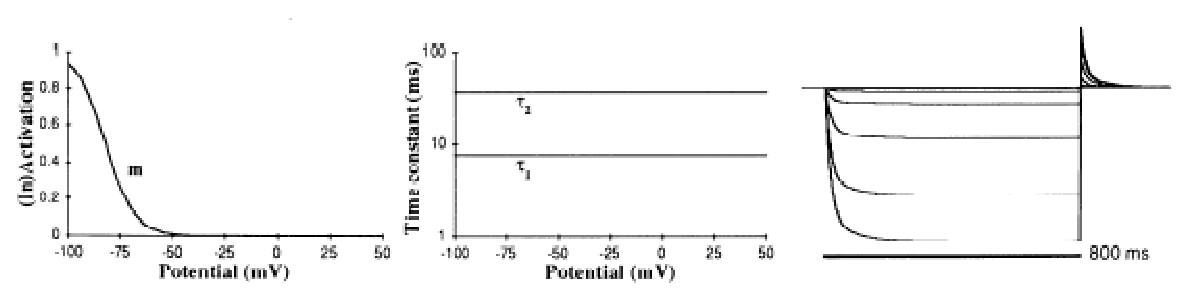
\includegraphics[scale=0.75]{figures/DS1.2D.eps}
   \caption{Activation and inactivation properties of the anomalous rectifier current (Kh, ---) in the model. Seady-state activation vs. voltage are plotted at the {\em left}, the time constants of activation ($\tau_1$ and $\tau_2$,) vs. voltage in the {\em middle} (Note: Semilogarithmic scale), and a simulation of representative voltage-clamp currents at the {\em right}. Note: This current does not inactivate and that activation is determined by 2 time constants\,\cite{Spain-W-J:1987ij}.}
   \label{fig:DS1.2D}
\end{figure}

\subsection*{Anomalous Rectifier Current (Kh)}

Inward rectification has been shown to be present in the Purkinje cell\,\cite{Crepel:1986cr, Hounsgaard:1988nx} and a channel permeable to K$^+$ and activated at hyperpolarized potentials has been identified in single-channel recordings (\cite{Gruol:1989oq}, K8). However, kinetic information on this channel for the Purkinje cell is incomplete. Accordingly, we have used the equations for the anomalous rectifier (Kh) in cortical neurons published by\,\cite{Spain-W-J:1987ij}. These equations have the same activation curve (Fig. 20) as the voltage-clamp data from a single Purkinje cell shown by\,\cite{Crepel:1986cr} (their Fig. 2).

\bibliographystyle{plain}
\bibliography{../tex/bib/g3-refs}

\end{document}
